\chapter{Defining the Research Scope: Questions, Challenges, and Data}

\section{Problem Statement and Research Question}
Social media platforms face significant challenges in managing toxic behavior, such as hate speech, harassment, and discrimination. While centralized platforms like Twitter have been extensively studied, decentralized alternatives like Mastodon present unique dynamics due to their federated architecture. Mastodon's distributed moderation system, where each instance operates independently, raises questions about how toxicity manifests and evolves across diverse communities.

This study aims to understand the evolution of toxicity on Mastodon over the entire year of~2024. Specifically, we address the following research question:

\begin{quote}
\textbf{How does toxicity vary across Mastodon instances, and how do instance-specific rules and moderation practices influence these patterns?}
\end{quote}

To answer this question, we conduct two experiments:

\begin{enumerate}
    \item \textbf{Toxicity Classifier Selection}: We evaluate three transformer-based toxicity prediction models to identify the most suitable one for our large-scale analysis.
    
    \item \textbf{Toxicity Detection and Analysis}: Using the selected model, we analyze a~1\% subsample of our dataset to detect toxic content and examine its distribution across instances. We further investigate how toxicity levels correlate with instance-specific rules and moderation practices.
\end{enumerate}

\section{Mastodon Dataset} \label{mastodon-dataset}
The dataset used in this study consists of public toots collected from a federated network of instances. The data was gathered using a distributed crawler developed by \citet{ernst:2024}, which collects toots from Mastodon instances' public timelines via their REST API while respecting user privacy settings. The crawler stores the collected data in an Elasticsearch cluster with careful attention to ethical considerations, never publishing raw user data.

\begin{figure}[tb]
    \centering
    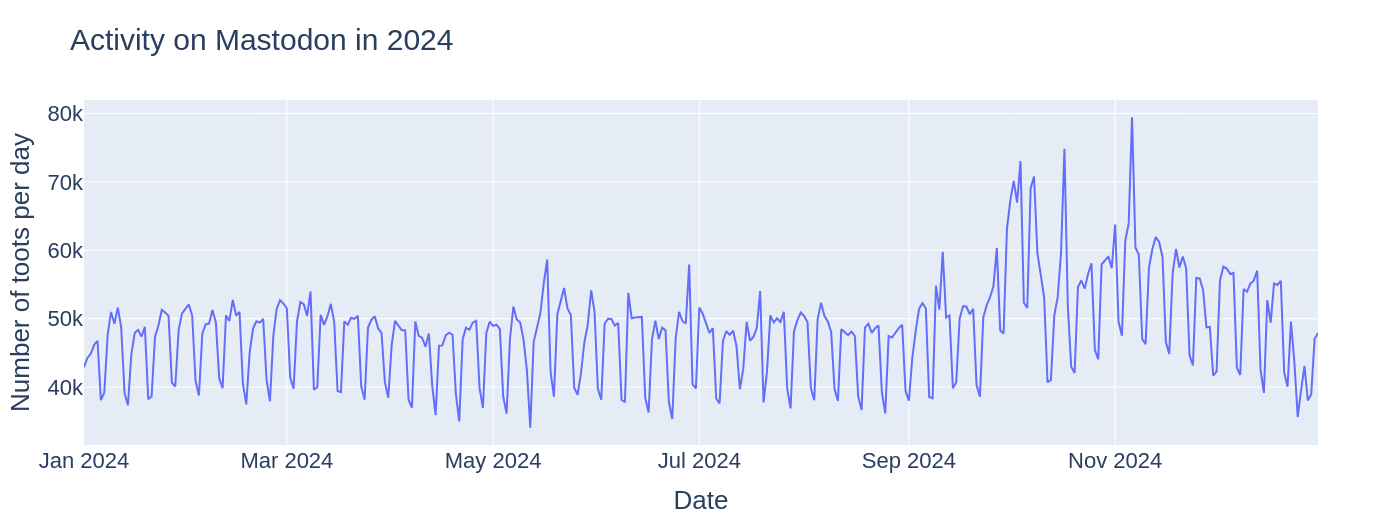
\includegraphics[width=\textwidth]{../material/activity_2024.png}
    \caption{Total number of toots in our subset per day.}
    \label{toot-distribution}
    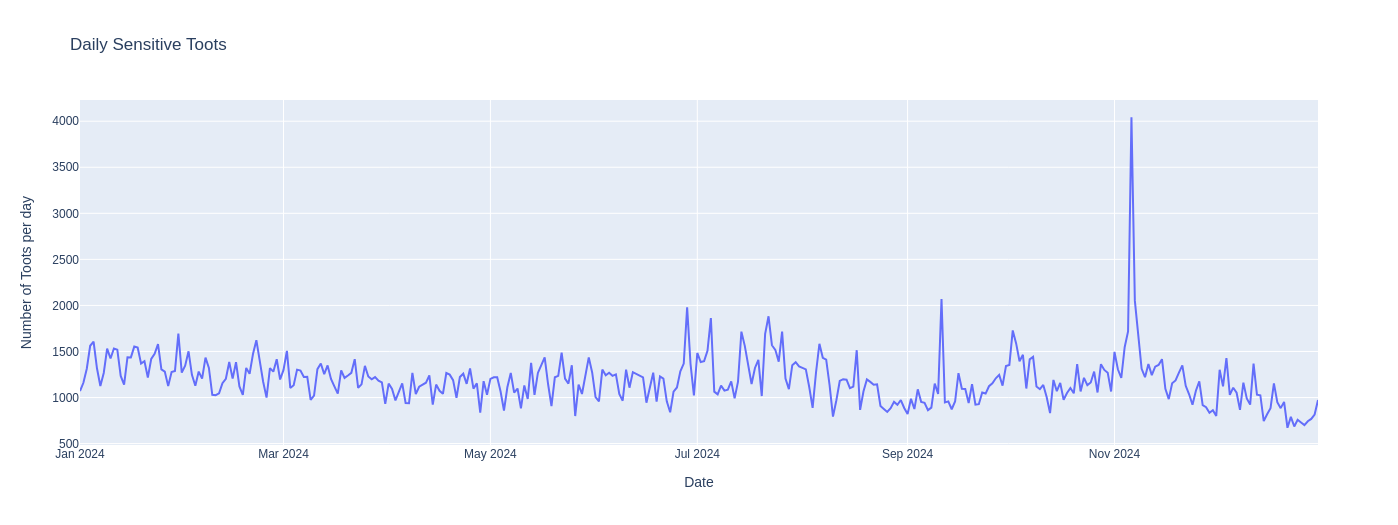
\includegraphics[width=\textwidth]{../material/sensitive_toots.png}
    \caption{Number of Toots marked as sensitive in our subset per day.}
    \label{sensitive-toots}
\end{figure}

As reported by \citet{ernst:2024} in November~2024, the corpus contained 3.6~billion toots collected over 301~days from 1,081~instances. The complete dataset includes detailed metadata about each toot and relationships between instances, with key fields described in Table~\ref{dataset-fields}. After deduplication, this resulted in 174~million unique toots, indicating a duplication rate of approximately 95\%, which reflects the federated nature of Mastodon where content is shared across instances. While the crawler has continued running since that report, our analysis focuses specifically on English-language toots from the complete year~2024, collected from 1,000~fully crawled instances.

\begin{table}[tb]
    \centering\small
    \renewcommand{\arraystretch}{1.3}
    \begin{tabularx}{\textwidth}{lX}
        \toprule
        \textbf{Field} & \textbf{Description} \\
        \midrule
        \texttt{id} & Unique identifier for each toot \\
        \texttt{content} & The toot content in HTML format (converted to plain text for analysis) \\
        \texttt{crawled\_from\_instance} & The instance where the toot was observed \\
        \texttt{instance} & The home instance of the posting user \\
        \texttt{is\_local} & Boolean indicating whether the toot originated on the crawled instance \\
        \texttt{created\_at} & Timestamp of toot creation \\
        \texttt{sensitive} & Flag marking potentially sensitive content \\
        \texttt{spoiler\_text} & Content warnings or spoiler alerts \\
        \bottomrule
    \end{tabularx}
    \caption{Key fields available in the Mastodon dataset with their descriptions.}
    \label{dataset-fields}
\end{table}

Approximately 18\% of toots contain media attachments (mostly images). Because our toxicity detection models just analyze text content, we removed those with media attachments. As well, we filtered out reblogs to reduce the dataset and focus on original toots. The final dataset contains around 1.8~billion toots

\begin{figure}[tb]
    \centering
    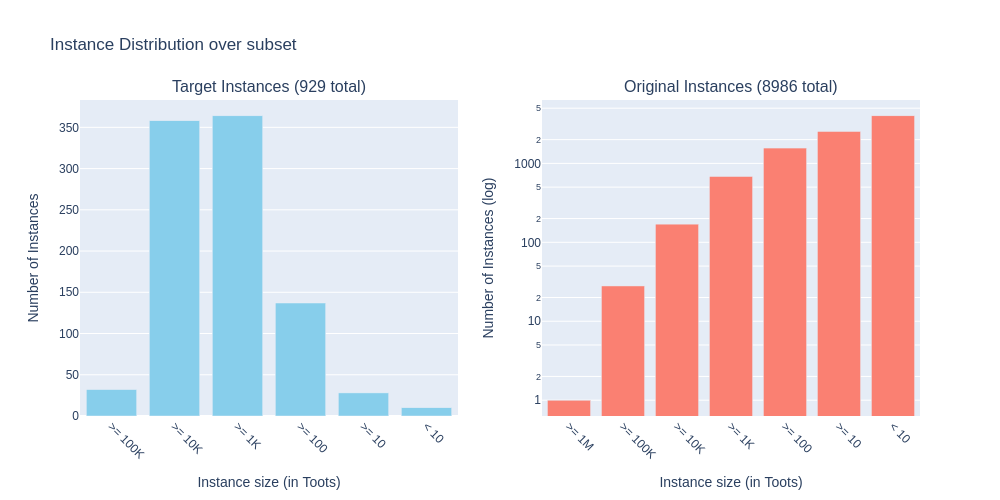
\includegraphics[width=\textwidth]{../material/instance_distribution.png}
    \caption{Distribution of Toot Counts per Instance: Comparison of Sources vs. Targets. The left chart shows the number of instances by toot volume for the target instances, while the right chart (log scale) shows the same for the source instances.}
    \label{instance-distribution}
\end{figure}

For our analysis, we use a~1\% subsample of the dataset, resulting in 17,691,031 toots. The subset is created by selecting 10 random toots from each batch of 1000. The batches cover a short time span, ensuring the timeline remains continuous. After subsampling, the subset exhibits the following key characteristics:

\begin{itemize}
\item 5.69\% of toots are flagged as sensitive content.
\item Approximately 20\% originate from users whose home instance is \textit{mastodon.social}.
\item While the origin of the toots is heavily centered on one instance (\textit{mastodon.social}), the distribution of the instances where the toots were posted is more balanced (see Figure~\ref{instance-distribution}).
\item During subsampling, 71 weakly represented instances were removed, leaving 929 instances.
\item The proportion of duplicates is reduced to 50\% (from 95\% in the original dataset).
\end{itemize}

As shown in Figure~\ref{toot-distribution}, the subsample maintains consistent temporal coverage throughout 2024. October and November saw an increase in the number of toots posted. This can be explained by the election campaign and the elections in the USA. There is also an extreme peak in toots marked as sensitive on the 6th of November 2024 (Figure~\ref{sensitive-toots}). As this was the first day after the election in the USA, Donald Trump's victory seems to be the reason. As \citet{zia:2023} already described, \textit{mastodon.social} dominates as users' home instance due to its size (Figure~\ref{instance-distribution}).